\chapter{Linux IoT Malware Classification}
\thispagestyle{chapterfancy}


Now that we verified the replicability of the model made by Wu \textit{et al.}, we ask ourselves the question: could the same ideas be applied to the classification of Linux IoT? \\
Before delving into the experimenting, we need to properly translate the steps performed in Chapter 4 to the Linux IoT environment. But even earlier than that, we need a dataset.

\section{Motivation}
With the rise in popularity of Internet of Things (IoT) devices, while our digital life has been made easier, our cybersecurity has been exposed to new threats, creating unprecedented challenges in safeguarding our personal information and ensuring the integrity of interconnected systems. \\
In particular, due to the open-sourceness of malware programs' code such as Mirai \cite{antonakakis2017understanding}, a botnet that took the Internet by storm in late 2016 when it overwhelmed several high-profile targets with massive distributed denial-of-service (DDoS) attacks, numerous malware variants have appeared, rendering the protection of IoT devices more challenging while also making it harder to disambiguate the ownership, lineage, and correct label of these malware variants. \\
Contrastive Learning is a technique that hasn't been employed many times in the IoT environment. To the best of our knowledge, only one paper uses (Self-supervised) Contrastive Learning for the classification of IoT Malware \cite{dib2022evoliot}. That said, its outstanding results in other fields make us confident about its capabilities. 

\section{CUBE-MALIOT-2021 Dataset}
Since IoT security hasn't been object of research for a long time, availability of datasets has been very scarce. However, it has now become more and more important to explore the cybersecurity of IoT devices, especially because they have been employed in many sensitive domains, including healthcare, transportation and agriculture. \\
After thorough research, we were able to gain access to a dataset, provided by CrySyS Lab and Ukatemi Technologies, called "CrySyS-Ukatemi BEnchmark: MALware for IOT devices 2021", or CUBE-MALIOT-2021\footnote{https://github.com/CrySyS/cube-maliot-2021} for short. The dataset consists of 29,209 ELF binaries compiled for the ARM platform and 18,715 ELF binaries compiled for the MIPS platform. \\
All metadata of the raw binaries is available as JSON documents, where the file name of each JSON document is the SHA256 hash of the corresponding malicious binary. These JSON documents contain information obtained from the binaries (e.g., ELF header information, file size, etc.) and information obtained from the VirusTotal\footnote{For more information, visit www.virustotal.com} analysis reports of the samples (e.g., first submission date to VirusTotal, antivirus labels assigned by antivirus products, etc.). Accurate antivirus labels were computed with a slightly modified version of AVClass (version 1) \cite{sebastian2016avclass}. \\

\begin{center}
\begin{lstlisting}[caption={Metadata of a Gafgyt ARM malware sample.}, captionpos=b, label={code:JSON}, language=json, xleftmargin=.03\textwidth, xrightmargin=.03\textwidth]
{
    "architecture": "ARM",
    "av_labels_generation_date": "2020-08-08T02:18:53",
    "avclass_labels": {
        "ddos": 3,
        "gafgyt": 14,
        "mirai": 2
    },
    "elf_header_info": {
        "abi_version": 0,
        "class": "ELF32",
        "data": "2's complement, little endian",
        "entrypoint": 33200,
        "hdr_version": "1 (current)",
        "num_prog_headers": 4,
        "num_section_headers": 24,
        "obj_version": "0x1",
        "os_abi": "UNIX - System V",
        "type": "EXEC (Executable file)"
    },
    "first_submission_date": "2017-03-11T17:23:29",
    "magic": "ELF 32-bit LSB executable, ARM, version 1 
              (SYSV), statically linked, not stripped",
    "magic_is_stripped": false,
    "magic_linking": "static",
    "md5": "356e84a502f1acd1f6363d17ce544312",
    "sha1": "3547c0c8030e93274fcf25c3701df0e8634ce682",
    "sha256": "0bbe52f239f903b9e922a795163e417dc1e1a3835b46
               22656bff46320adb0ef2",
    "size": 134804,
    "tlsh": "91D30A05D8509737C2D22BBAF7AA42CE73261FA8579733
             1296287EF41FE1B9D1D39120"
}
\end{lstlisting}
\end{center}

\pagebreak 

\noindent In the Code Listing \ref{code:JSON} is shown the JSON file of an ARM malware sample. To properly divide our dataset between malware families, we write a simple python script that puts each malware in the family that has the highest AVClass score in its JSON. Following this procedure, the malware described in Code Listing \ref{code:JSON} would be classified as a Gafgyt malware.

\section{Static Analysis for ELF files}
In the previous chapter we worked with APK (Android Package) files, a format used to distribute and install applications on the Android operating system. Now that we've moved to the Linux Environment we'll be working with ELF (Executable and Linkable Format) files, a format used for executables on Unix and Unix-like operating systems. \\
Because of this, we need a new way to extract the Function Call Graph from the malware samples. To do so, we will use Radare2, an open-source framework for reverse engineering and binary analysis. \\
The analysis of a malware would proceed as follows:

\begin{center}
\begin{adjustbox}{width=0.94\linewidth,keepaspectratio}
\begin{lstlisting}[style=Radare2]
C:\Users\Sandman\Desktop>r2 0013b477ce0de71e48076e36217baf4f3dc5e4a325210d17320a178a41a584d4
[0x00008194]> aaa
INFO: Analyze all flags starting with sym. and entry0 (aa)
WARN: Cannot find basic block for switch case at 0x000106a4 bbdelta = 12
INFO: Analyze all functions arguments/locals (afva@@@F)
INFO: Analyze function calls (aac)
INFO: Analyze len bytes of instructions for references (aar)
INFO: Finding and parsing C++ vtables (avrr)
INFO: Finding xrefs in noncode section (e anal.in=io.maps.x)
INFO: Analyze value pointers (aav)
INFO: aav: 0x00008000-0x0001aee8 in 0x8000-0x1aee8
INFO: Emulate functions to find computed references (aaef)
INFO: Type matching analysis for all functions (aaft)
INFO: Propagate noreturn information (aanr)
INFO: Integrate dwarf function information
INFO: Use -AA or aaaa to perform additional experimental analysis
[0x00008194]> afl
0x00008194    1     44 entry0
0x000080f0    3     48 sym.__do_global_dtors_aux
0x00008134    1     32 sym.frame_dummy
0x0000d6bc    1     16 sym.anti_gdb_entry
0x0000d6d4    1     64 sym.resolve_cnc_addr
0x000113dc    4    152 sym.table_unlock_val
0x00012a54    1     40 sym.inet_addr
0x000188cc   17    240 sym.inet_aton
0x00011318    1     32 sym.table_retrieve_val
0x0001133c    4    152 sym.table_lock_val
0x0000e1dc    3    196 sym.setup_connection
0x00015760    3    100 sym.__GI_close
0x00015a08   16    212 sym.__libc_enable_asynccancel
0x00015980   11    136 sym.__libc_disable_asynccancel
0x00012f98    3     60 sym.socket
0x00016190    1     16 sym.__aeabi_read_tp
0x000119b0    3     36 sym.util_zero
0x00012038    9    228 sym.__libc_fcntl
0x00012b04    3    108 sym.connect
0x00012ac0    3     60 sym.__sys_connect
0x0000e2a4    7    340 sym.add_auth_entry
0x000122dc    3     64 sym.__syscall_select
0x000125f0    5    200 sym.fd_to_DIR
0x00012c44    3     60 sym.__sys_recv
0x00012cf8    3     68 sym.__sys_recvfrom
0x00012dc8    3     60 sym.__sys_send
0x00012e7c    3     68 sym.__sys_sendto
...
\end{lstlisting}
\end{adjustbox}
\end{center}

\noindent The \texttt{r2} command launches the Radare2 interactive command-line interface (CLI) and opens the specified binary file for analysis. We then use the \texttt{aaa} command to trigger a series of automatic analyses to gather information about the binary, including identifying functions, creating basic blocks, and recognizing data structures. We can use the \texttt{afl} command to list all the functions in the analyzed binary to have a better understanding of its behaviour. A subset of these functions will take the place of the API calls in the previous chapter image generation. \\
This framework also gives us access to the generation of multiple graphs: 

\begin{center}
\begin{lstlisting}[style=Radare2,escapechar=\%,xleftmargin=.1\textwidth, xrightmargin=.03\textwidth]
[0x00008194]> ag?
Usage: ag<graphtype><format> [addr]
%\color{darkpastelgreen}Graph commands:%
| aga[format]             %\color{darkpastelgreen}data references graph%
| agA[format]             %\color{darkpastelgreen}global data references graph%
| agc[format]             %\color{darkpastelgreen}function callgraph%
| agC[format]             %\color{darkpastelgreen}global callgraph%
| agd[format] %\color{goldenpoppy}\bfseries[fcn addr]%    %\color{darkpastelgreen}diff graph%
| agf[format]             %\color{darkpastelgreen}basic blocks function graph%
| agi[format]             %\color{darkpastelgreen}imports graph%
| agr[format]             %\color{darkpastelgreen}references graph%
| agR[format]             %\color{darkpastelgreen}global references graph%
| agx[format]             %\color{darkpastelgreen}cross references graph%
| agg[format]             %\color{darkpastelgreen}custom graph%
| agt[format]             %\color{darkpastelgreen}tree map graph%
| ag-                     %\color{darkpastelgreen}clear the custom graph%
| agn[?] title body       %\color{darkpastelgreen}add a node to the custom graph%
| age[?] title1 title2    %\color{darkpastelgreen}add an edge to the custom graph%

%\color{darkpastelgreen}Output formats:%
| <blank>                 %\color{darkpastelgreen}ascii art%
| *                       %\color{darkpastelgreen}r2 commands%
| b                       %\color{darkpastelgreen}braile art rendering (agfb)%
| d                       %\color{darkpastelgreen}graphviz dot%
| g                       %\color{darkpastelgreen}graph Modelling Language (gml)%
| j                       %\color{darkpastelgreen}json ('J' for formatted disassembly)%
| k                       %\color{darkpastelgreen}sdb key-value%
| m                       %\color{darkpastelgreen}mermaid%
| t                       %\color{darkpastelgreen}tiny ascii art%
| v                       %\color{darkpastelgreen}interactive ascii art%
| w [path]                %\color{darkpastelgreen}write to path or display graph image%
\end{lstlisting}
\end{center}

\noindent The one that we need is the "global callgraph". After a few tests, we landed on graphviz dot as the best output format. Using the command \texttt{agCdw} we save the .gv file of the global callgraph. \\
Using r2pipe, a set of libraries that provide a way to interact with Radare2 through various programming languages, we can automate the creation of these graphs for all of our malware samples with a simple python script.

\section{Sensitive Functions List}
When creating a Global callgraph with Radare2, the nodes of the graph will have either “fcn.” or “sym.” as prefix. The “fcn.” nodes represent UDFs (User Defined Functions), while “sym.” modes represent Library Functions declared in the header of the binary. In graph form, since we are studying the behaviour of the malware based on the nodes names, UDFs don't give us any information, so our only focus will be Library functions.

\begin{figure}[H]
    \centering
    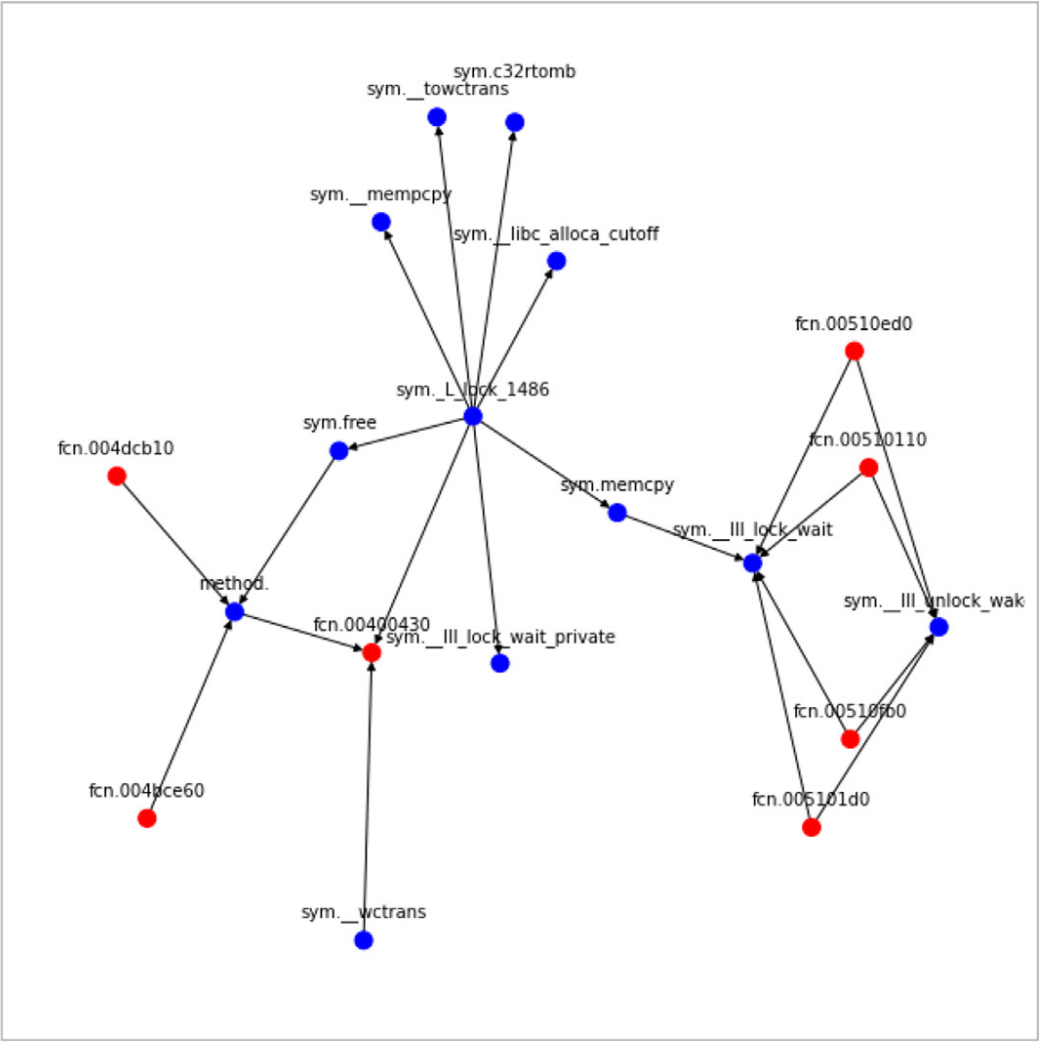
\includegraphics[width=0.7\linewidth]{Images/ELFGraph.png}
    \caption{Example of a Function Call Graph extracted using Radare2. The red nodes are UDFs, while the blue nodes are Library functions.}
    \label{fig:ELFGraph}
\end{figure}

\noindent Our objective now is to find a set of Library functions that are able to correctly describe the malicious behaviour of a program. Differently from Android, there haven't been many studies on the most used libraries by malware families. That said, we did find a study \cite{akabane2021identification} analyzing the most common toolchains used to build Linux IoT malware (Table \ref{tab:Toolchains}), \textit{i.e.} a set of tools that compiles source code into executables that can run on a target device. It includes a compiler (a tool that translates high-level source code into machine code), a linker (a program that takes one or more object files (generated by a compiler or an assembler) and combines them into a single executable file), and run-time libraries (collections of precompiled routines, functions, and procedures). \\
In their research, they found out that most Linux malware are built with toolchains using well-known toolchain building tools available in binary form online, rather than customized toolchains for anti-analysis.

\begin{table}[H]
    \centering
    \resizebox{0.94\linewidth}{!}{
    \begin{tabular}{|c|c|}
        \hline
        Building tool: toolchain components & Number of samples \\
        \hline\hline
        Firmware Linux 0.9.6 : GCC 4.1.2, binutils 2.17, uClibc 0.9.30.1 & 3,830 \\
        \hline
        Aboriginal Linux 1.1.0 : GCC 4.2.1, binutils 2.17, uClibc 0.9.32 & 8 \\
        \hline
        Aboriginal Linux 1.1.1 : GCC 4.2.1, binutils 2.17, uClibc 0.9.32.1 & 6 \\
        \hline
        Aboriginal Linux 1.2.0 : GCC 4.2.1, binutils 2.17, uClibc 0.9.33.2 & 17 \\
        \hline
        Aboriginal Linux 1.2.1 : GCC 4.2.1, binutils 397a64b3, uClibc 0.9.33.2 & 11 \\
        \hline
        Aboriginal Linux 1.2.4 : GCC 4.2.1, binutils 397a64b3, uClibc 0.9.33.2 & 27 \\
        \hline
        Aboriginal Linux 1.2.6 : GCC 4.2.1, binutils 2.17, uClibc 0.9.33.2 & 22 \\
        \hline
        Aboriginal Linux 1.4.3 : GCC 4.2.1, binutils 397a64b3, uClibc 0.9.33.2 & 6 \\
        \hline
        Aboriginal Linux 1.4.4 : GCC 4.2.1, binutils 2.17, musl 1.1.12 & 36 \\
        \hline
        Buildroot 2018.08 (Bootlin toolchain) : GCC 7.3.0, binutils 2.29.1, uClibc-ng 1.0.30 & 22 \\
        \hline
        Buildroot 2018.08 (Bootlin toolchain) : GCC 7.3.0, binutils 2.29.1, musl 1.1.19 & 2 \\
        \hline
        Buildroot 2018.08 (Synopsys toolchain) : GCC 7.1.1, binutils2.29, uClibc-ng 1.0.26 & 2 \\
        \hline
        Crosstool-NG 1.24.0-rc1: GCC 8.2.0, binutils 2.30, musl 1.1.19 & 2 \\
        \hline
    \end{tabular}
    }
    \caption{Result of toolchain identification performed by Akabane \textit{et al.} \cite{akabane2021identification}.}
    \label{tab:Toolchains}
\end{table}

\noindent By using these findings, we can focus on the "run-time libraries" portion of the toolchains to be able to list the most common library functions found in Linux IoT malware. As shown in Table \ref{tab:CLibraries}, the most used C Library in Linux IoT malware is uClibc, a small and lightweight C library designed for embedded systems and systems with limited resources. \\

\begin{table}[H]
    \centering
    \begin{tabular}{|c|c|c|}
    	\hline
        C library & Number of samples & Percentage \\
        \hline\hline
        uClibc & 3,951 & 99.00\% \\
        \hline
        musl & 40 & 1.00\% \\
        \hline
    \end{tabular}
    \caption{Most used C libraries by malware samples as found by Akabane \textit{et al.} \cite{akabane2021identification}.}
    \label{tab:CLibraries}
\end{table}

\noindent We decided to focus on the functions in the uClibc 0.9.30.1, since it's the version contained in the most commonly used toolchain (Firmware Linux 0.9.66, which is described in the Mirai installation guide  \cite{anna2016mirai}). This way, we restricted ourselves to 2214 library functions, which will constitute our "sensitive" functions list. \\
Unfortunately, a problem arises due to the fact that many IoT malware samples includes static linking of library functions, and their symbols such as function names and addresses are stripped, hindering function-level analysis. A way to solve this problem has been proposed by Akabane and Okamoto in "Identification of library functions statically linked to Linux malware without symbols" \cite{akabane2020identification} and will be discussed later in this chapter. For the sake of this thesis, we'll work on the unstripped malware samples present in the CUBE-MALIOT-2021 Dataset.

\section{Results}
It’s now time to train our new model. This time, we will generate 95*95 pixel grayscale image (with a 169 pixels padding, since $95*95-2214*4=169$) following the same criteria as \textit{IFDroid}. We used once again both a NVIDIA Tesla T4 (provided by Leonardo S.p.A.) and a NVIDIA GeForce RTX 3050 interchangeably for this experiment. We also use the same Parameters for both the encoder and the classifier as \textit{IFDroid}. \\
We reduced the dataset to the 3 malware families with the most unstripped samples: \textsc{Gafgyt}, \textsc{Mirai} and \textsc{Ddostf}. These malware families target and compromise IoT devices, turning them into a botnet used for large-scale distributed denial-of-service (DDoS) attacks. In total we'll use 1000 \textsc{Gafgyt} samples, 1000 \textsc{Mirai} samples and 707 \textsc{Ddostf} samples. \\
We train our model for 100 epochs both both our encoder and our classifier. At epoch 0, the encoder has a train loss of 4.06207 and a validation loss of 4.14268, while at epoch 99 it has a train loss of 3.12014 and a validation loss of 3.21261. Our classifier, on the other hand, at epoch 0 has a train loss of 1.11393 and a validation loss of 1.10900, while at epoch 99 it has a train loss of 0.29114 and a validation loss of 0.29571.

\begin{figure}[H]
    \centering
    \begin{subfigure}{0.45\textwidth}
        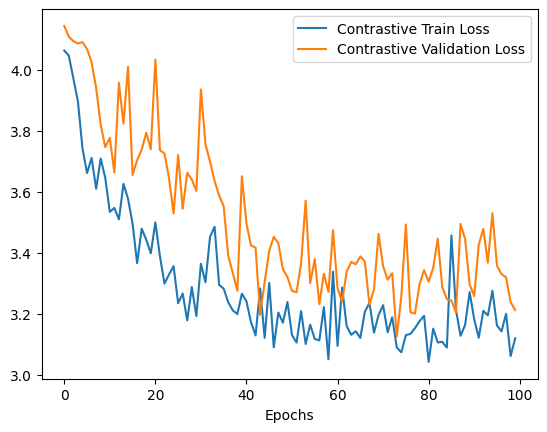
\includegraphics[width=\linewidth]{Images/ConLoss_IoT.png}
        \caption{Encoder Loss}
        \label{fig:ConLossIoT}
    \end{subfigure}
    \hfill
    \begin{subfigure}{0.45\textwidth}
        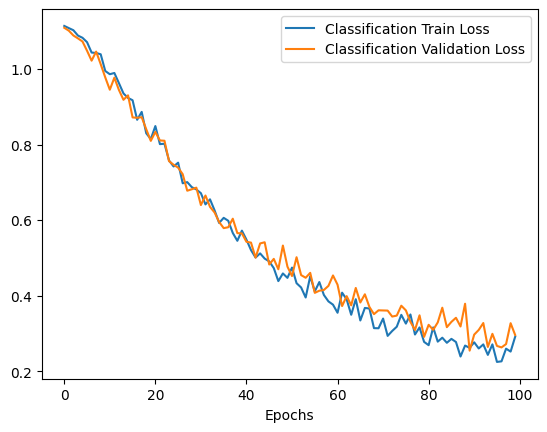
\includegraphics[width=\linewidth]{Images/ClassLoss_IoT.png}
        \caption{Classifier Loss}
        \label{fig:ClassLossIoT}
    \end{subfigure}
    \caption{Variation of the Loss over the epochs for the IoT encoder and classifier.}
    \label{fig:LossIoT}
\end{figure}

\noindent In Table \ref{tab:IoTVS} we show some widely used metrics (Table \ref{tab:Metrics}) to measure the effectiveness of our model.

\begin{table}[H]
    \centering
    %\resizebox{\linewidth}{!}{
    \begin{tabular}{|c|c|c|c|c|c|c|}
        \hline
    \textbf{Family} & \textbf{TPR(\%)} & \textbf{FPR(\%)} & \textbf{F1Score} & \textbf{Accuracy} & \textbf{Precision} & \textbf{Recall} \\
        \hline
        gafgyt & 100 & 0.0 & 100 & 100 & 100 & 100 \\
        mirai & 87.5 & 0.0 & 93.3 & 87.5 & 100 & 87.5 \\
        ddostf & 100 & 6.2 & 91.8 & 100 & 84.8 & 100 \\
        \hline
    \end{tabular}
    %}
    \caption{Result metrics of our IoT malware classifier.}
    \label{tab:IoTVS}
\end{table}

\noindent Last but not least, we show some metrics improvements of our model over the epochs.

\begin{figure}[H]
    \centering
    \begin{subfigure}{0.3\textwidth}
        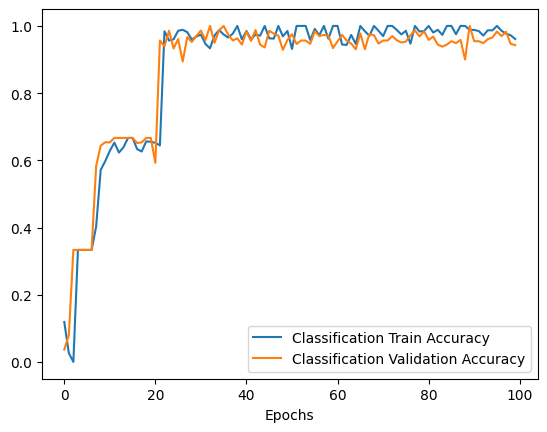
\includegraphics[width=\linewidth]{Images/Acc_IoT.png}
        \caption{Accuracy}
        \label{fig:AccuracyIoT}
    \end{subfigure}
    \hfill
    \begin{subfigure}{0.3\textwidth}
        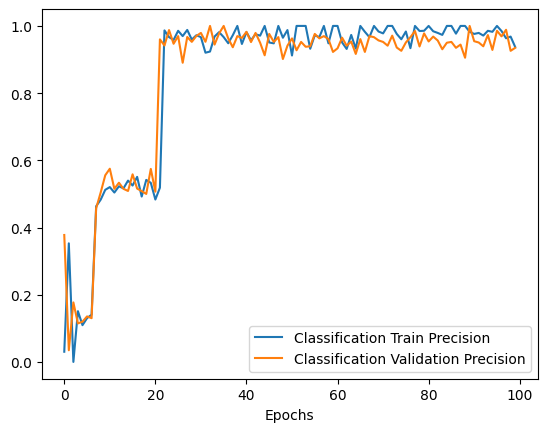
\includegraphics[width=\linewidth]{Images/Prec_IoT.png}
        \caption{Precision}
        \label{fig:PrecisionIoT}
    \end{subfigure}
    \hfill
    \begin{subfigure}{0.3\textwidth}
        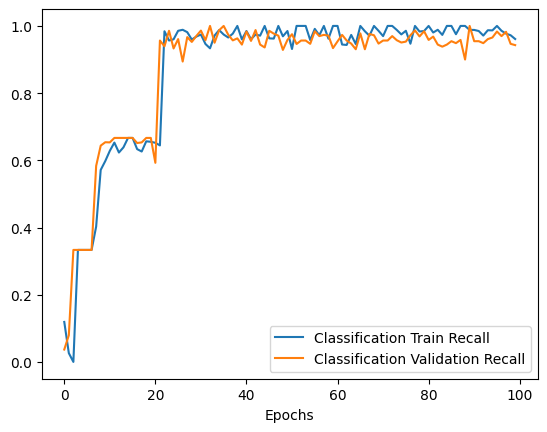
\includegraphics[width=\linewidth]{Images/Rec_IoT.png}
        \caption{Recall}
        \label{fig:RecallIoT}
    \end{subfigure}
    \caption{Variation of different effectiveness metrics over the epochs for the IoT classifier.}
    \label{fig:MetricsIoT}
\end{figure}

\section{Conclusions}
Even while working with only a small amount of samples, the neural network was able to achieve great results in the classification of these malware families. That being said, many compromises where made to be able to reach those results, especially focusing only on unstripped samples. \\
There exists a few different ways to identify a stripped function:

\begin{itemize}
    \item \textbf{IDA F.L.I.R.T} \cite{hex2015idaflirt}: checks, at each byte of the program being disassembled, whether it can mark the start of a standard library function. Each function is represented by a pattern, the first 32 bytes of a function where all variant bytes (\textit{i.e.}, bytes that don't have any relevance in the identification of the function) have a special character, and the CRC16 (cyclic redundancy check) of the bytes starting from position 33 until the first variant byte. However, since modern real-world libraries contain several functions starting with the same bytes and the checksum is only computed until the first variant byte appears, unique matching of C library functions isn't guaranteed to be achieved.
    \item \textbf{FCatalog} \cite{xorpd2015fcatalog}: identifies a function by comparing its instruction sequences to a database. It can identify a function even if the order of instructions differ or an instruction is replaced with an alternative. However, they may falsely identify different functions as being the same if they have the same sequence of instructions but different registers.
    \item \textbf{BinDiff} \cite{dullien2005graph}: identifies a function by comparing control flow graphs of two functions. They are tolerant to instruction replacement and sequence reordering in a node of the control flow graph, but they may falsely identify different functions as being the same if they have the same control flow graph.
    \item \textbf{BinSequence} \cite{huang2017binsequence}: combines instruction sequence similarity and control flow graph similarity to identify functions. May also falsely identify different functions as being the same if a pair of functions have a similar sequence of instructions or similar control flow graphs. 
\end{itemize}

\noindent Function identification by pattern matching is difficult because compiler-generated machine code differs for each toolchain. Moreover, function identification based on the similarity of machine code and/or its control flow graph gives false results if two different functions have the same sequence of instructions but different registers or different immediate data. In fact, many C library functions result in false positives for this reason. \\
Due of these problems, Akabane and Okamoto conducted some accurate studies \cite{akabane2020identification}\cite{akabane2021identification} focusing on library functions recognition for Linux IoT malware. \\
Because of the high diversity of C libraries for desktop computers and servers, pattern matching for identification of these library functions requires generation of various patterns from a large number of libraries. This requires a lot of time and effort. In contrast, there are few C libraries for embedded devices, and fewer versions. Furthermore, their study has confirmed that malware developers prefer toolchains built with Firmware Linux series \cite{landley2002firmware}. \\
Their results showed that pattern matching identified toolchains used to build 97.7\% of 2,256 samples with the Intel 80386 architecture, indicating that pattern matching is indeed effective for function identification of Linux malware on embedded devices.
